\chapter{Descripción del hardware}\label{chp-02}

\lettrine[lraise=-0.1, lines=2, loversize=0.2]{U}na vez conocidas las funciones
que debe desempeñar el sistema es importante definir el hardware a usar para que
sea capaz de cumplimentar los requerimientos establecidos. Los principales dispositivos
utilizados en el proyecto son los siguientes:

\section{Arduino Mega 2560}

Se trata de una placa de desarrollo que cuenta con el microcontrolador ATmega2560 y todo lo
necesario para prototipar un sistema. Cuenta con 54 pines de entrada y salida (GPIO), de los cuales
15 pueden utilizarse como salida PWM, 4 puertos UART, oscilador de 16 MHz, conexión USB tipo B,
pines ICSP de programación y botón de reinicio.

\begin{figure}[hbtp]
	\centering
	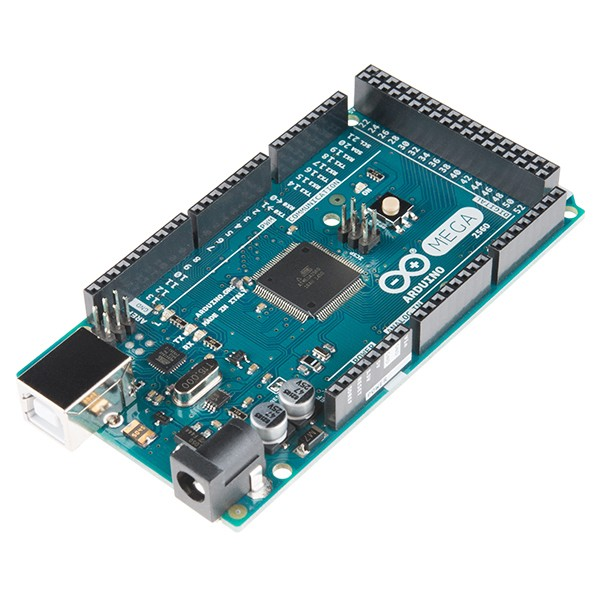
\includegraphics[scale=0.5]{02-hardware/01-arduino-mega-2560.jpg}
	\caption{Arduino Mega 2560}
	\label{fig:figura2}
	\end{figure}


\begin{table}[hbtp]
    \begin{center}
    \begin{tabular}{ | c | c |  }
    \hline
    Microcontrolador & ATmega2560 \\ \hline
    Tensión de funcionamiento & 5 V \\ \hline
    Voltaje de entrada recomendado & 7-12 V \\ \hline
    Voltaje de entrada límite & 6-20 V \\ \hline
    Pines de E/S digitales & 54 (de los cuales 15 con salida PWM) \\ \hline
    Pines de entrada analógica & 16 \\ \hline
    Corriente CC por pin & 20 mA \\ \hline
    Corriente CC para pin 3.3 V & 50 mA \\ \hline
    Memoria Flash & 256 kB, 8 kB utilizados por el gestor de arranque \\ \hline
    SRAM & 8 kB \\ \hline
    EEPROM & 4 kB \\ \hline
    Frecuencia de reloj & 16 MHz \\ \hline
    Longitud & 101.52 mm \\ \hline
    Anchura & 53.3 mm \\ \hline
    Peso & 37 g \\ \hline

    \end{tabular}
    \end{center}
    \caption{Características Arduino Mega 2560}
    \label{tab:tab1}
    \end{table}


\subsection{Alimentación}

El Arduino Mega 2560 puede ser alimentado mediante la conexión USB tipo B proporcionada por
un ordenador o por una fuente de alimentación externa. Además, puede ser alimentado por los pines
de alimentación de la placa, que se describen a continuación:

\begin{itemize}
    \item VIN. Entrada de tensión de la placa cuando hay alimentación externa.
    \item 5V. Pin que produce 5V regulados.
    \item 3V3. Pin que produce 3.3V regulados con un consumo máximo de 50 mA.
    \item GND. Pin de conexión a masa.
    \item IOREF. Referencia de tensión de trabajo del microcontrolador.
\end{itemize}

\subsection{Memoria}

El ATmega2560 cuenta con 256 kB de memoria flash de los cuales 8 kB se usan para el gestor de arranque,
8 kB de memoria SRAM y 4 kB de EEPROM.

\subsection{Entradas y Salidas}

El Arduino Mega cuenta con 54 pines que pueden ser utilizados como salida o entrada digital mediante
las funciones pinMode(), digitalWrite() y digitalRead(). Los niveles lógicos son de 5V. Cada pin soporta
una corriente de 20 mA y cuenta con una resistencia de pull-up de entre 20 y 50 k$\Omega$. Además, algunos pines
tienen funciones especiales:

\begin{itemize}
    \item Comunicación serie. Se usa para recibir y transmitir datos en serie TTL. Son las parejas 0 y 1,
    14 y 15, 16 y 17 y 18 y 19. Los pines 0 y 1 son los correspondientes a la comunicación con el conversor 
    USB-TTL integrado en la placa
    \item Interrupciones externas. Se utilizan para activar interrupciones en el software. Son los pines 2, 3, 18, 19, 20 y 21.
    \item Salida PWM. Proporcionan una salida modulada con 8 bits de precisión con la función analogWrite(). Son los pines del 
    2 al 13 y del 44 al 46.
    \item Comunicación SPI. Pines 50 (MISO), 51 (MOSI), 52 (SCK), 53 (SS). Permiten comunicación SPI con otros 
    dispositivos utilizando la biblioteca SPI.
    \item LED integrado. En el pin 13 hay un LED integrado que puede encenderse con un valor HIGH y apagarse con un valor LOW.
    \item Comunicación TWI. Pines 20 (SDA) y 21 (SCL). Permite comunicación I2C/TWI.
\end{itemize}

\subsection{Comunicación}

La placa Arduino Mega cuenta con diversas formas para comunicarse con un ordenador o con otros dispositivos. El ATmega2560
cuenta con cuatro UART de hardware para comunicación TTL a 5V, una conexión SPI y una conexión I2C. Mediante uno de los puertos
UART el ATmega2560 se comunica con un ATmega16U2 que canaliza la conexión mediante USB a un ordenador y permite la comunicación
entre ambos. Esto permite tanto programar la placa mediante el IDE de Arduino como recibir mediante monitor serie datos simples.

\section{Ethernet Shield de Arduino}



\section{Motor DC y Driver L298N}

\subsection{Conexionado del módulo L298N}

\section{Encoder Rotativo Incremental}

\subsection{Especificaciones técnicas}

\subsection{Conexionado del Encoder}

\section{Calibrador digital}

\section{LCD}

\section{Sensor fotoeléctrico OMRON}

\section{Banda transportadora con elementos integrados}

\section{Controlador IRC5C}